% Reproducible architecture figure for the implemented W2 decaying-turbulence core.
% Source invariants: 256^2 DNS -> sharp spectral filter -> 64^2 coarse state;
% channel-first float32 (1,64,64); ETDRK2; 822,977 flattened CNN parameters;
% operator split omega_{t+1} = omega_tilde + dt C_theta(omega_tilde).
% Implementation sources (repository root):
% src/tesseract_hybrid_closure/{data,components,losses,tesseract_components}.py
% tesseracts/{coarse_solver,scalar_closure}/tesseract_api.py
\documentclass[tikz,border=4pt]{standalone}
\usepackage[T1]{fontenc}
\usepackage{helvet}
\renewcommand{\familydefault}{\sfdefault}
\usepackage{amsmath,amssymb}
\usepackage{xcolor}
\usepackage{tikz}
\usetikzlibrary{arrows.meta,backgrounds,calc,fit,positioning}

% Okabe--Ito colour-blind-safe palette.
\definecolor{Orange}{HTML}{E69F00}
\definecolor{SkyBlue}{HTML}{56B4E9}
\definecolor{Green}{HTML}{009E73}
\definecolor{Blue}{HTML}{0072B2}
\definecolor{Vermillion}{HTML}{D55E00}
\definecolor{Purple}{HTML}{CC79A7}
\definecolor{Charcoal}{HTML}{303030}

\begin{document}
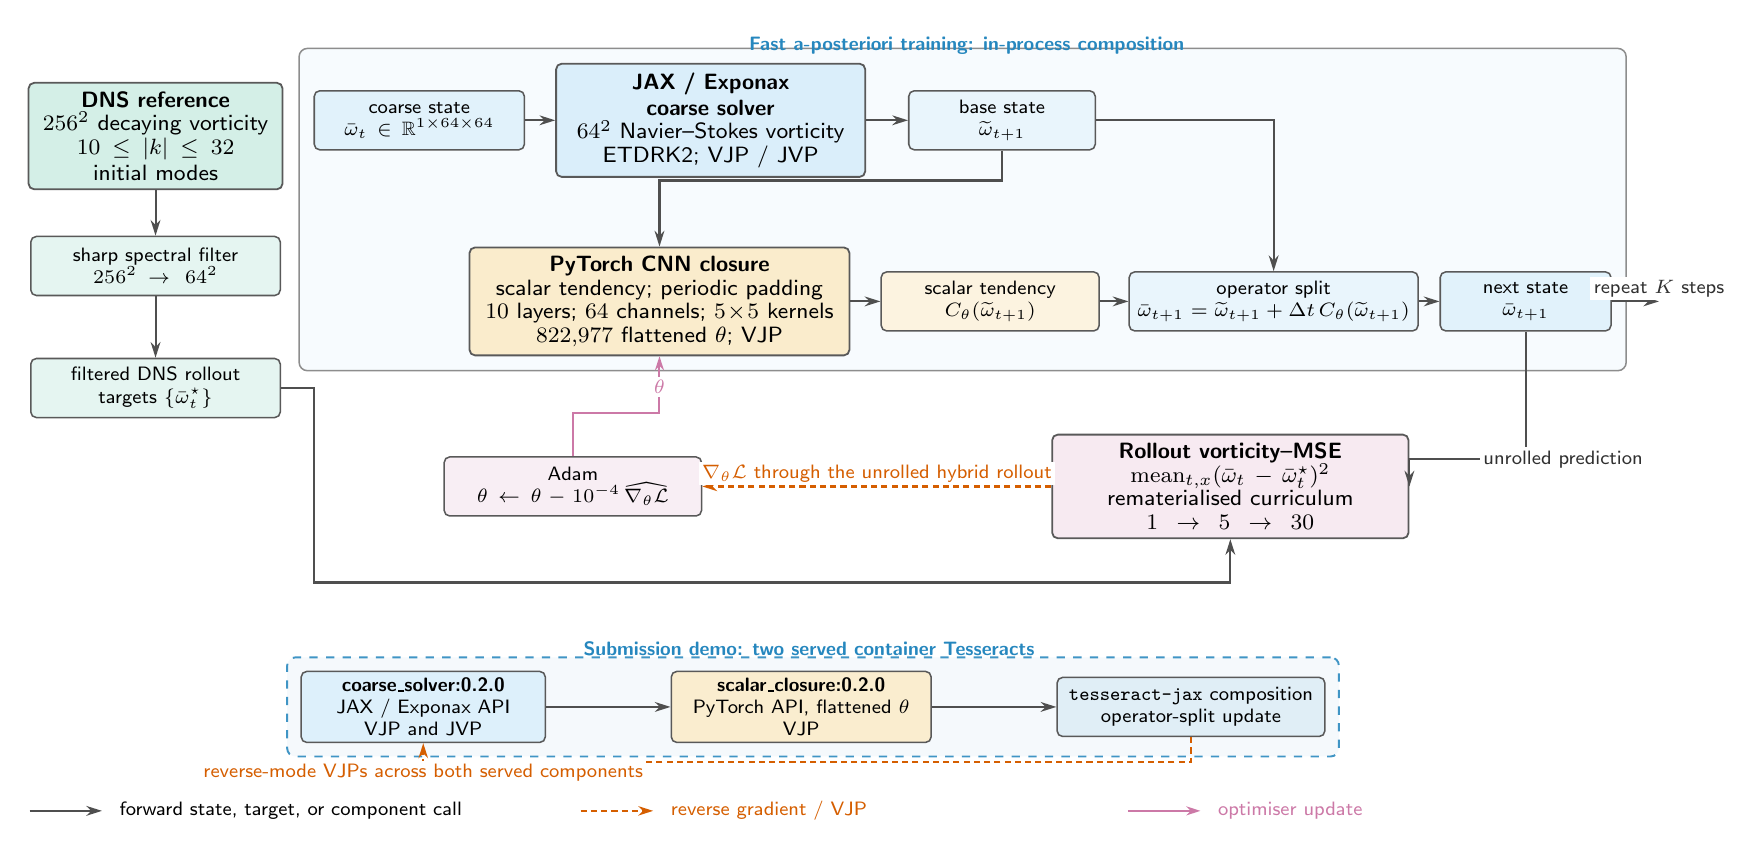
\begin{tikzpicture}[
  x=1cm, y=1cm,
  font=\footnotesize,
  box/.style={rounded corners=2pt, draw=Charcoal!80, line width=.65pt,
    minimum height=10mm, align=center, inner sep=3.2pt},
  smallbox/.style={rounded corners=2pt, draw=Charcoal!80, line width=.55pt,
    minimum height=7.5mm, align=center, inner sep=2.4pt, font=\scriptsize},
  flow/.style={-{Stealth[length=2.0mm,width=1.25mm]}, line width=.75pt, draw=Charcoal!85},
  grad/.style={-{Stealth[length=1.9mm,width=1.2mm]}, dashed, dash pattern=on 2.2pt off 1.5pt,
    line width=.78pt, draw=Vermillion},
  update/.style={-{Stealth[length=1.8mm,width=1.15mm]}, line width=.72pt, draw=Purple},
  label/.style={font=\scriptsize, fill=white, inner sep=1.2pt, text=Charcoal},
  group/.style={rounded corners=3pt, draw=Charcoal!55, line width=.55pt, fill=SkyBlue!5,
    inner sep=5.2pt},
  demo/.style={rounded corners=3pt, draw=Blue!75, dashed, line width=.7pt, fill=Blue!4,
    inner sep=4.8pt}
]

% Reference trajectory generation is deliberately separate from the training loop.
\node[box, fill=Green!17, minimum width=30mm, text width=30mm] (dns) at (1.8,6.15)
  {\textbf{DNS reference}\\[-1pt]
   $256^2$ decaying vorticity\\[-1pt]
   $10\leq |k|\leq32$ initial modes};
\node[smallbox, fill=Green!10, minimum width=30mm, text width=30mm] (filter) at (1.8,4.50)
  {sharp spectral filter\\$256^2\!\rightarrow64^2$};
\node[smallbox, fill=Green!10, minimum width=30mm, text width=30mm] (targets) at (1.8,2.95)
  {filtered DNS rollout\\targets $\{\bar\omega_t^\star\}$};
\draw[flow] (dns) -- (filter);
\draw[flow] (filter) -- (targets);

% Fast training path: a two-row operator-split rollout.
\node[smallbox, fill=SkyBlue!18, minimum width=25mm, text width=25mm] (state) at (5.15,6.35)
  {coarse state\\$\bar\omega_t\in\mathbb{R}^{1\times64\times64}$};
\node[box, fill=SkyBlue!22, minimum width=37mm, text width=37mm] (solver) at (8.85,6.35)
  {\textbf{JAX / Exponax coarse solver}\\[-1pt]
   $64^2$ Navier--Stokes vorticity\\[-1pt]
   ETDRK2; VJP / JVP};
\node[smallbox, fill=SkyBlue!13, minimum width=22mm, text width=22mm] (base) at (12.55,6.35)
  {base state\\$\widetilde\omega_{t+1}$};

\node[box, fill=Orange!20, minimum width=46mm, text width=46mm] (closure) at (8.20,4.05)
  {\textbf{PyTorch CNN closure}\\[-1pt]
   scalar tendency; periodic padding\\[-1pt]
   $10$ layers; $64$ channels; $5\!\times\!5$ kernels\\[-1pt]
   $822{,}977$ flattened $\theta$; VJP};
\node[smallbox, fill=Orange!12, minimum width=26mm, text width=26mm] (tendency) at (12.40,4.05)
  {scalar tendency\\$C_\theta(\widetilde\omega_{t+1})$};
\node[smallbox, fill=SkyBlue!13, minimum width=35mm, text width=35mm] (split) at (16.00,4.05)
  {operator split\\$\bar\omega_{t+1}=\widetilde\omega_{t+1}+\Delta t\,C_\theta(\widetilde\omega_{t+1})$};
\node[smallbox, fill=SkyBlue!18, minimum width=20mm, text width=20mm] (next) at (19.20,4.05)
  {next state\\$\bar\omega_{t+1}$};

\draw[flow] (state) -- (solver);
\draw[flow] (solver) -- (base);
\draw[flow] (base.south) -- ++(0,-.38) -| (closure.north);
\draw[flow] (base.east) -- ++(.50,0) -| (split.north);
\draw[flow] (closure) -- (tendency);
\draw[flow] (tendency) -- (split);
\draw[flow] (split) -- (next);
\draw[flow] (next.east) -- ++(.60,0) node[above, label]{repeat $K$ steps};

% Objective and parameter update.  Routes stay below the forward computation.
\node[smallbox, fill=Purple!13, minimum width=31mm, text width=31mm] (adam) at (7.10,1.70)
  {Adam\\$\theta\leftarrow\theta-10^{-4}\,\widehat{\nabla_\theta\mathcal{L}}$};
\node[box, fill=Purple!16, minimum width=43mm, text width=43mm] (loss) at (15.45,1.70)
  {\textbf{Rollout vorticity--MSE}\\[-1pt]
   $\operatorname{mean}_{t,x}(\bar\omega_t-\bar\omega_t^\star)^2$\\[-1pt]
   rematerialised curriculum\\[-1pt]
   $1\rightarrow5\rightarrow30$};
\draw[flow] (targets.east) -- ++(.42,0) |- ($(loss.south)+(0,-.55)$) -- (loss.south);
\draw[flow] (next.south) -- ++(0,-1.62) -| node[pos=.20, right, label]{unrolled prediction} (loss.east);
\draw[grad] (loss.west) -- node[above, label, text=Vermillion]
  {$\nabla_\theta\mathcal{L}$ through the unrolled hybrid rollout} (adam.east);
\draw[update] (adam.north) -- ++(0,.55) -| node[pos=.83, below, label, text=Purple]{$\theta$} (closure.south);

\begin{scope}[on background layer]
  \node[group, fit=(state)(solver)(base)(split)(next)(closure)(tendency)] {};
\end{scope}
\node[font=\scriptsize\bfseries, text=Blue!85] at (12.10,7.30)
  {Fast a-posteriori training: in-process composition};

% Containerised submission-demo path remains separate from the fast training path.
\node[smallbox, fill=SkyBlue!20, minimum width=31mm] (demoSolver) at (5.20,-1.10)
  {\textbf{coarse\_solver:0.2.0}\\JAX / Exponax API\\VJP and JVP};
\node[smallbox, fill=Orange!19, minimum width=33mm] (demoClosure) at (10.00,-1.10)
  {\textbf{scalar\_closure:0.2.0}\\PyTorch API, flattened $\theta$\\VJP};
\node[smallbox, fill=Blue!12, minimum width=34mm] (demoCompose) at (14.95,-1.10)
  {\texttt{tesseract-jax} composition\\operator-split update};
\draw[flow] (demoSolver) -- (demoClosure);
\draw[flow] (demoClosure) -- (demoCompose);
\draw[grad] (demoCompose.south) -- ++(0,-.31) -|
  node[pos=.55, below, label, text=Vermillion]{reverse-mode VJPs across both served components}
  (demoSolver.south);
\begin{scope}[on background layer]
  \node[demo, fit=(demoSolver)(demoClosure)(demoCompose)] {};
\end{scope}
\node[font=\scriptsize\bfseries, text=Blue!85] at (10.10,-.36)
  {Submission demo: two served container Tesseracts};

% Legend.
\draw[flow] (.20,-2.42) -- (1.12,-2.42);
\node[anchor=west, font=\scriptsize] at (1.22,-2.42) {forward state, target, or component call};
\draw[grad] (7.20,-2.42) -- (8.12,-2.42);
\node[anchor=west, font=\scriptsize, text=Vermillion] at (8.22,-2.42) {reverse gradient / VJP};
\draw[update] (14.15,-2.42) -- (15.07,-2.42);
\node[anchor=west, font=\scriptsize, text=Purple] at (15.17,-2.42) {optimiser update};
\end{tikzpicture}
\end{document}
